\chapter{Related Works}
\label{chap:relatedworks}

In this chapter we provide a general overview on the different approaches that are taken into account in order to provide a reliable, secure, and transparent communication between on-premise application's layers and off-premise Cloud data stores. Furthermore, we discuss about the needed adaptations different authors specify that the on-premise application's layers must address when migrating their underlying layers to a Cloud infrastructure. We compare it to the ones we transparently support in our approach, and the ones the user should consider. We finally mention the improvements we need to perform to the original prototype ServiceMix-mt, and continue our discussion dividing it into the two main \ac{DBMS} available nowadays in the market: \ac{SQL} and \ac{NoSQL} databases.

%% non functional data layer patterns paper: make a big emphasis on the proxy approach. It is quite similar to our approach, because it allows horizontal scalability between different target data sources, but there is no need of abstracting the proxy from the database layer. esb's are horizontally scalable and can form a esb cluster, as described in the esb part in fundamentals. we can have in our approach a bottleneck when using one instance of the esb. furthermore, their proxy approach assumes that the database layer is in the private cloud, while in ours the database layer can reside either on or off premise.
A migration process of the Database Layer of an application to the Cloud may pop up several incompatibilities with the new hosting environment, which need to be addressed prior to the migration decision. Strauch et al. aim to address such incompatibilities by defining a set of \term{Cloud Data Patterns}, which target finding a solution for a challenge related to the data layer of an application in the Cloud for a specific context \cite{strauchABKL2012}. Incompatibilities a user may find when migrating the application's data layer can be on the level of the schema representation, supported set of queries or query language, communication protocol, security, etc. Strauch et al. focus mainly in two non-functional aspects: enabling data store scalability and ensuring data confidentiality \cite{strauchABKL2012}. 

The former deals with maintaining the quality of service levels when the workload increases, for both write and read operations. There are two scalability mechanisms when dealing with data: vertical and horizontal scalability. A vertical scalable system can be obtained by introducing more powerful hardware, or moving to a more powerful database system, while a horizontal scalable system deals with splitting data into groups which are stored in different partitions or different database systems, also known as \term{sharding}. Due to the absence of support for accessing a \term{sharded database} between different database systems, the concepts of a database proxy and sharding-based router are introduced. In this first approach, a proxy component is locally added below each data access layer \cite{strauchABKL2012}. A proxy below each data access layer instead of a common proxy on top of the database layer dismisses a common point of failure when accessing the data. In the second approach, a local sharding-based router is added below each of the data access layer. A sharded-based router contains the needed knowledge about the location of the \term{sharded databases}. In our approach, we don't only partially follow both of the concepts, but integrate them in a single component. We consider a sharded-based router as a proxy with routing capabilities. Therefore, as it is discussed in Chapter \ref{chap:design}, enhancing an \ac{ESB} with the required \term{sharded databases} knowledge and with standardized communication protocols, it allows us to utilize it as a sharded-based router, and as a proxy. Furthermore, the single point of failure avoidance can be ensured by increasing the number of \ac{ESB} instances and balancing the load between them. As discussed before, we do not fully comply with this approach. The development of a proxy or sharded-based router component below each data access layer forces each application to deploy at least one proxy or sharded-router instance in their system. In our approach we propose the utilization of our prototype as a shared transparent Cloud data access layer by connecting to a data access endpoint which supports a specific \ac{DBMS} multi-tenant aware communication protocol (e.g. MySQL or PostgreSQL). For this purpose, we propose the concept of a lightweight Data Layer, where the adaptations to its sublayers are minimized, e.g. modification of data access host, port, etc. The data access endpoint acts as a database protocol-aware proxy, forwarding the requests to the \ac{NMR} of the \ac{ESB}. We enhance the Myosotis Tungsten Connector and provide access control, caching functionality, and full integration in the \ac{ESB} \ac{OSGi} container, and with the \ac{NMR} \cite{tungstenwiki}.

%% Data confidentiality between the on premise app layers and the migration layers and how can we still ensure data confidentiality: mention the 5 patterns that are in steve's article. Mention that this article gives a deep focus on security patterns rather than technical information regarding the router between the data stores. we do not implement automatic data filtering for confidentiality. the user is the one who decides which data goes off premise and which data stays in premise. we provide support for off premise and on the on premise data. however, this can be reached in our esb but requires user customization, in order to be able to filter data per user and to route it to the appropriate data store.

Ensuring data confidentiality is presented in \cite{strauch2012}. Their work deals with critical data management between on-premise and off-premise data stores, and categorizes data into different confidentiality levels to prevent data disclosures. The former is achieved by aggregating information which categorizes data into different categories and confidentiality levels. The latter deals with keeping confidential data on-premise. With data filtering, pseudonymization, and anonymization, data is either prevented from being externally routed, or secured when routed to a public Cloud \cite{strauch2012}. The pseudonymization technique provides to the exterior a masked version of the data while maintaining its relation with the original data, and the anonymization provides to the exterior a reduced version of the data. In this diploma thesis' approach, we assume that the application's owner has decided on which data should be and cannot be migrated, and that the business layer is hosted on-premise. Therefore, there is no data processing in a public Cloud environment. Our final prototype provides confidentiality between different tenants of the system by injecting tenant information  in our messages and providing tenant-aware routing, and different multi-tenant aware endpoints. We do not need to provide support for pseudonymization or anonymization techniques, in contrast to \cite{strauch2012}.

%% table of what do i have to do when migrating app or app components to the cloud. this is from the book chapter of vasilios and steve. comment here what ive written in the comments
Replacement of components which build an application with Cloud offerings leads the developers to face an application's adaptation process. For example, migrating a local database to a private Cloud or to a public Cloud, or sharding a database between on-premise and off-premise data stores forming a single data store system, can not be accessible without adapting the non-migrated application's layers to the new storage system. Andrikopoulos et al. identify the needed adaptations actions when migrating a data layer to the Cloud \cite{andrikopoulos2013}: address reconfiguration, patterns realization, incompatibilities resolution, query transformation, and interaction with data store allowance. Our main goal in our final prototype is to minimize the number of adaptations the user must perform when migrating application's data to a Cloud data store. The adaptations of the \ac{ESB} must encompass the described adaptations in a transparent way to the user, in order to internally support in our prototype compatibility between the application and the different data stores, and lower the adaptation operations number at the application's side, e.g. only address reconfiguration. 

%% speak a little bit about federated databases
%% have taken notes in the paper. the main thing to say here is the main difference between a federated database system and our approach. Our approach works more or less than a federated database system, but more like a federated server, where transparent access to backend datasources is provided. joins are out of the scope of the thesis. indicate that one main component in a federated dbs is the transformer, in our case between sql databases, and between nosql databases, but this is out of scope of this thesis. 
%% mediator in page 37 of the book principles of distributed database systems
Federated Database Systems are a type of \ac{MDBS} that allow accessing and storing data which is stored in different and noncontiguous databases through a single interface. Sheth and Larson define them as a collection of cooperating but autonomous component database systems, which can be integrated to various degrees, and can be accessed by a software which controls and coordinates the manipulation of the database systems which conforming the federated database system. This distributed database model allows users to access and store data among different database systems, which can be located in different continents, without dealing with multiple connections to the different database systems, query and data transformation, address adaptation, etc. \ac{MDBS} are accessed through a single endpoint which provides a single logical view of the \ac{MDBS}, and users can access the different \ac{DBMS} which form the \ac{MDBS} (see Figure \ref{fig:multidatabasesystem}). 

\begin{figure}[htb]
	\centering
		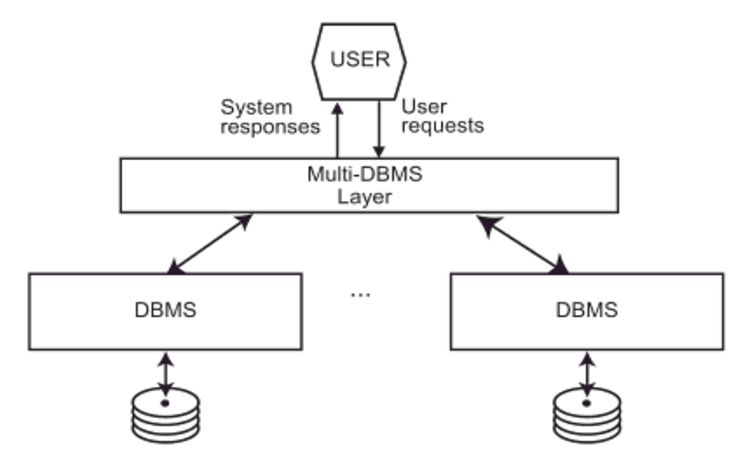
\includegraphics[clip, scale=0.6]{./gfx/multidatabasesystem.pdf}
	\caption[Multidatabase System Components]{Components in a multidatabase system \cite{ddbsozsu}}
	\label{fig:multidatabasesystem}
\end{figure}

A popular implementation architecture for a \ac{MDBS} is the mediator/wrapper approach \cite{ddbsozsu}. Mediators exploits knowledge to create information for upper layers, while wrappers provide mapping between different views, e.g. relational vs. object-oriented views. We can consider our approach as a \ac{MDBS} with some modifications and less functionalities. In the first place, using the \ac{ESB} as a single entrance point to the data system while managing different backend autonomous Cloud or traditional data stores comply with the main concept of a \ac{MDBS}. Furthermore, Cloud data store providers may implement the same distributed database model, whereby we could find two logical levels for accessing the physical data. However, we do not accurately follow the mediator/wrapper approach. In our approach we exploit data provided by the tenant during the migration decision and process, by providing an interface to register the backend data store/s information in our system, for future routing purposes. Furthermore, compatibility information is registered in order to apply the needed query or data transformation between data stores. However, the transformation is out of the scope of this diploma thesis, and the support of table joins between databases located in different Cloud data stores are out of scope as well.
%%tenant isolation approach in muhler versus tenant and user isolation approach in this work. explain the granularity of tenant and users, one tenant may want to migrate his database to a data store, but in this case one database can have one or more users. it is not like in muhlers approach where tenants are considered applications accessing the esb. 

As described in the previous chapter, multi-tenancy is one of the main requirements in a Cloud environment. Muhler, Essl, and Gomez provide an extended version of ServiceMix 4.3, which supports multi-tenancy at two different levels: communication, and administration and management \cite{Muhler2012}, \cite{Essl2011}, \cite{gomez2012}. However, their prototype supports tenant isolation at the level of tenants. A \ac{DBMS}, e.g. MySQL, by default provides access to one default user and supports multiple users creation \cite{mysqlmanual}. Therefore, in our approach we must not only consider isolation at the tenant level, but also at the user level. We assume that the tenant is the default user which migrates his data store to a Cloud environment, but the migrated data store may contain one or more users. In our prototype we ensure tenant and user isolation at both communication, and administration and management levels.

%% caching mechanism used in our approach, explaining the two levels of caching that we use. compare it to the actual mysql proxy and to the databases architectures in the cloudcomputingdatabaseapps paper, say that caching is not discussed in their approach. caching applies for both mysql and nosql. drivers provided by the different vendors do not provide caching functionality. caching functionality must be trated in the application or in the server. caching is good not only for performance, but also to give the possibility to reduce costs in the tenants data stores in the cloud. most of the providers dont only charge per storage size, but also per calls to their api
%%mention the paper
%% put examples on amazon pricing : Micro DB Instance	$0.025 Small DB Instance	$0.090 Medium DB Instance	$0.180 Large DB Instance	$0.365 Extra Large DB Instance	$0.730 this are prices of usage per hour
%% amazon dynamo db: Write Throughput: $0.01 per hour for every 10 units of Write Capacity - Read Throughput: $0.01 per hour for every 50 units of Read Capacity
%% google cloud storage: (per 1,000 requests/month) PUT, POST, GET bucket**, GET service** Requests $0.01 - GET, HEAD Requests (per 10,000 requests/month) $0.01 - DELETE Requests free
Over the past decades, caching has become the key technology in bridging the performance gap across memory hierarchies via temporal or spatial localities; in particular, the effect is prominent in disk storage systems \cite{cashing2012}. Han et al. investigate how cost efficiency in a Cloud environment can be achieved, specially in applications which require a high I/O activities number, and present a CaaS (cache-as-a-service) model. Cloud providers offering data storage solutions present pricing models based on the storage size, usage per time, or number of requests. Amazon RDS costs \$0.025 per hour for a Micro DB Instance usage  \cite{amazonrds}, while Amazon DynamoDB \$0.01 per hour for every 50 units of read capacity \cite{amazondynamodb}, and Google Cloud Storage \$0.01 per 1000 PUT, POST, GET requests per month \cite{googlecloudstorage}. An I/O-intensive application whose database is hosted in the Cloud may produce a significant economic cost. The cost of continuously retrieving data from the Cloud data store, when existing temporal proximity between the data accessed, can be considered unnecessary, and reducible. Furthermore, the application's overall performance can be reduced due to the network latency and, in the scope of this work, the use of an \ac{ESB} to access the Cloud data store. In this diploma thesis we do not provide cashing as a service, but include cashing support to the sharded-based router pattern described in \cite{strauchABKL2012}. Uralov enhaces ServiceMix-mt with cashing support for dynamic discovery and selection of Cloud data hosting solutions \cite{Uralov2012}. However, we must adapt and extend it due to the lack of support of functionalities we require and the lack of full \ac{OSGi} compliance. 

\section{SQL Support Architectural Overview}
\label{sec:designsql}

In this section we provide an overview of a preliminary, and final architectural approaches designed in this diploma thesis, in order to support a transparent data access to backend \ac{SQL} databases. We first expose the integration approaches we should consider, and the main problems found when implementing the first approach which led us to design a second architectural approach. 


\subsection{Integration}

%integration of osgi and jbi in terms of messaging
%integration of osgi and jbi in terms of containers and libraries
%explain why we have two approaches
%jbi components offered in servicmix are deployed as osgi bundles
% jbi components offered in servicemix-mt are deployed as jbi component, and internally wrapped into an osgi bundle
% may have to put a figure of the contents in both of the packages so that we can see. It is all about the meta inf library where the bundle manifest info is exposed
As described in Chapter \ref{chap:spec}, we build the new components in ServiceMix-mt following the \ac{OSGi} compliance. However, these must interact with components which follow the \ac{JBI} specification. The integration between components built for different containers in ServiceMix-mt must be done at two levels: messaging, and resources sharing. The ServiceMix-mt \ac{NMR} \ac{API} \ac{OSGi} bundle exposes a set of operations for sending messages through the \ac{NMR} to a specified target endpoint. Hereby we can perform message exchanges between endpoints configured on \ac{OSGi} bundles and endpoints configured on \ac{JBI} components, and provide communication support between components hosted in the two containers. 

\begin{figure}[htb]
	\centering
		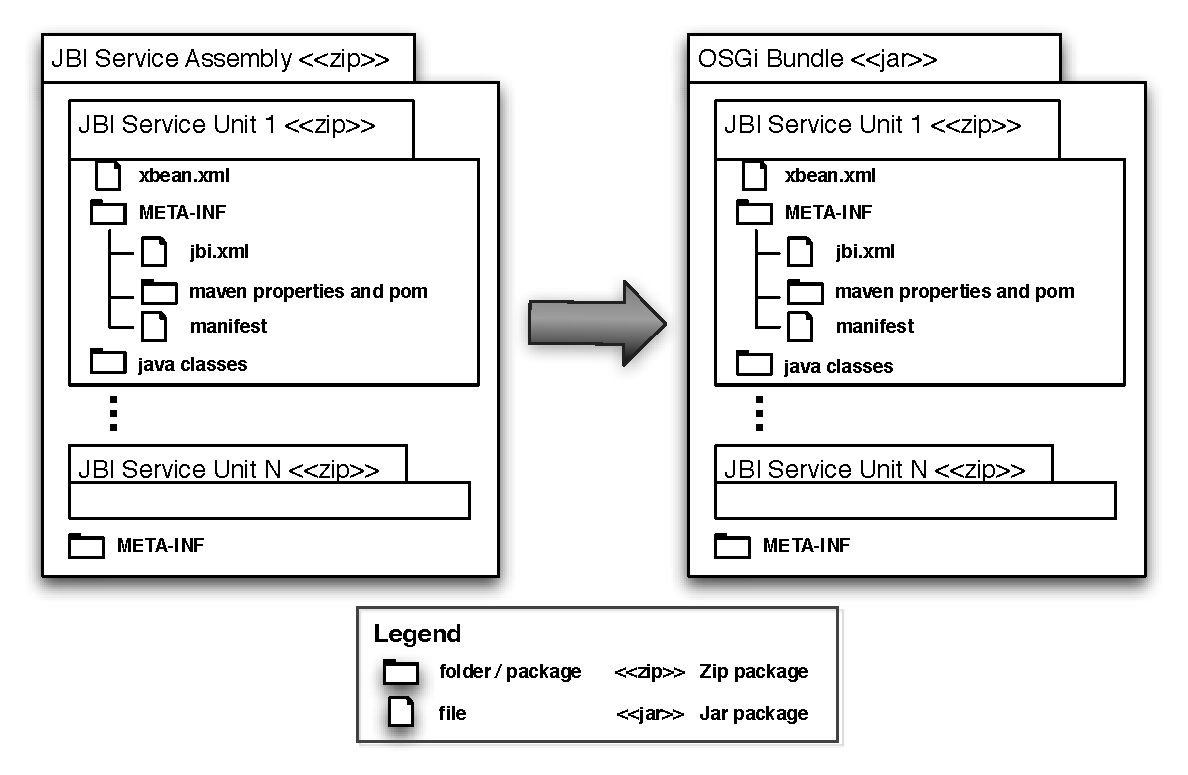
\includegraphics[clip, scale=0.5]{./gfx/osgibundlepackage.pdf}
	\caption[JBI to OSGi repackaging]{ServiceMix 4.x repackaging mechanism for deploying \ac{JBI} components in \ac{OSGi} container.}
	\label{fig:jbitoosgipackage}
\end{figure}

The resources sharing integration level refers to the deployment of \ac{JBI} components in the \ac{OSGi} container, and the utilization of packages exposed by \ac{OSGi} bundles in the \ac{OSGi} container in a loosely coupled manner. The former is part of the integration between containers provided in ServiceMix 4.x versions and described in Figure \ref{fig:jbitoosgipackage}. The deployment mechanism of a \ac{JBI} \ac{SA} into an \ac{OSGi} container is simple: repackaging of the \ac{SA} as a JAR. However, this cannot be consider a full integration in the \ac{OSGi} container. \ac{OSGi} bundles contain in their \term{META-INF} folder one fundamental file for the \ac{OSGi} kernel: the \term{manifest} file. This contains a description of the bundle, the packages it imports, and exports. Imported packages can be either statically stored in the bundle or imported from third party bundles, and exported packages are the ones which exposed to third party bundles. These can be imported with an internal class loading mechanisms developed in the \ac{OSGi} container. The repackaging of the \ac{SA} into a JAR, as it is shown in Figure \ref{fig:jbitoosgipackage}, contains the \term{META-INF} folder, and the \term{manifest} file. However, the latter only contains information about the author, date of creation, but it does not contain information related to the exported packages, and the needed packages to be imported. This \term{manifest} file describes the \ac{SA}, and not the \ac{SU}s. Java classes and package importing description are contained in the \ac{SU} package, and not in the \ac{SA} package. Therefore, the \ac{OSGi} container cannot register in its registry the packages it exports as a service, and cannot load the imported packages to the bundle context. This fact forces us to statically include in the \ac{SA}, and the \ac{SU} the packages which are referenced in each \ac{SU}, and leads to scalability constraints with the tenant-aware deployment process of the system.

ServiceMix 4.x versions are shipped with different \ac{JBI} \ac{BC}s packed as an \ac{OSGi} bundle. However, they are deployed as \ac{OSGi} bundles, and not as \ac{SA}s, in order to enable loose coupling and package sharing between components in the \ac{OSGi} container. ServiceMix-mt allows the deployment of the \ac{JBI} \ac{BC}s, but deployment of \ac{JBI} \ac{BC}s as OSGi bundles is not supported in the JBIMulti2 application. This lack of support forces us to design a second architectural approach, as described in the following sections.

\FloatBarrier

\subsection{Approach 1}

\ac{SQL} database systems provide access to their databases through an endpoint, which is represented as an URL. The native driver used in the data access layer of an application connects to the endpoint, authenticates, sends the query, and reads the response. Therefore, we must support in our system the same operational steps. As discussed in this diploma thesis, the communication protocol varies between different vendors. In this diploma thesis we provide support for incoming MySQL messages. Tenants must access our system through a single physical endpoint. This endpoint is provided by a MySQL proxy which is enriched with authentication, cashing, marshaling, and demarshaling operations. As shown in Figure \ref{fig:designsqlapp1}, the MySQL Proxy Bundle implements the MySQL server operations which are related with the client/server communication protocol. In Figure \ref{fig:designsqlapp1} we specify a server running on port 3306. However, this value can be configured before the deployment of the \ac{OSGi} component. This component is built as an \ac{OSGi} bundle and its packages are exported as services in the \ac{OSGi} container. It interacts with three different components in the system: the \ac{NMR} \ac{API}, the Cache, and the Service Registry. 

Cashing mechanisms are implemented in both the Registry-Cache, and the MySQL Proxy Bundle. The former provides an \ac{API} for creating cache instances, and for persisting and retrieving data. We create a separate cache instance for the \ac{SQL} support due to the need of a custom key creation mechanism which may not coexist in a shared cache between different bundles, as well as the needed isolation of sensible tenant configuration information from third party bundles. The system provides a set of operations which ease the creation of multi-tenant aware keys for persisting frontend authentication data, and queries results form the backend database systems. 

The \ac{NMR} \ac{API} is shipped in ServiceMix as an \ac{OSGi} bundle which exports its \ac{API} as an \ac{OSGi} service. The set of operations included in its \ac{API} allows \ac{OSGi} bundles to create, send, and receive message exchanges to \ac{JBI} endpoints (see Figure \ref{fig:designsqlapp1}).  Before creating the message exchange, the MySQL Proxy Bundle must build dynamically the target endpoint's URL by injecting the tenant context information, and service and endpoint name.

\begin{figure}[htb]
	\centering
		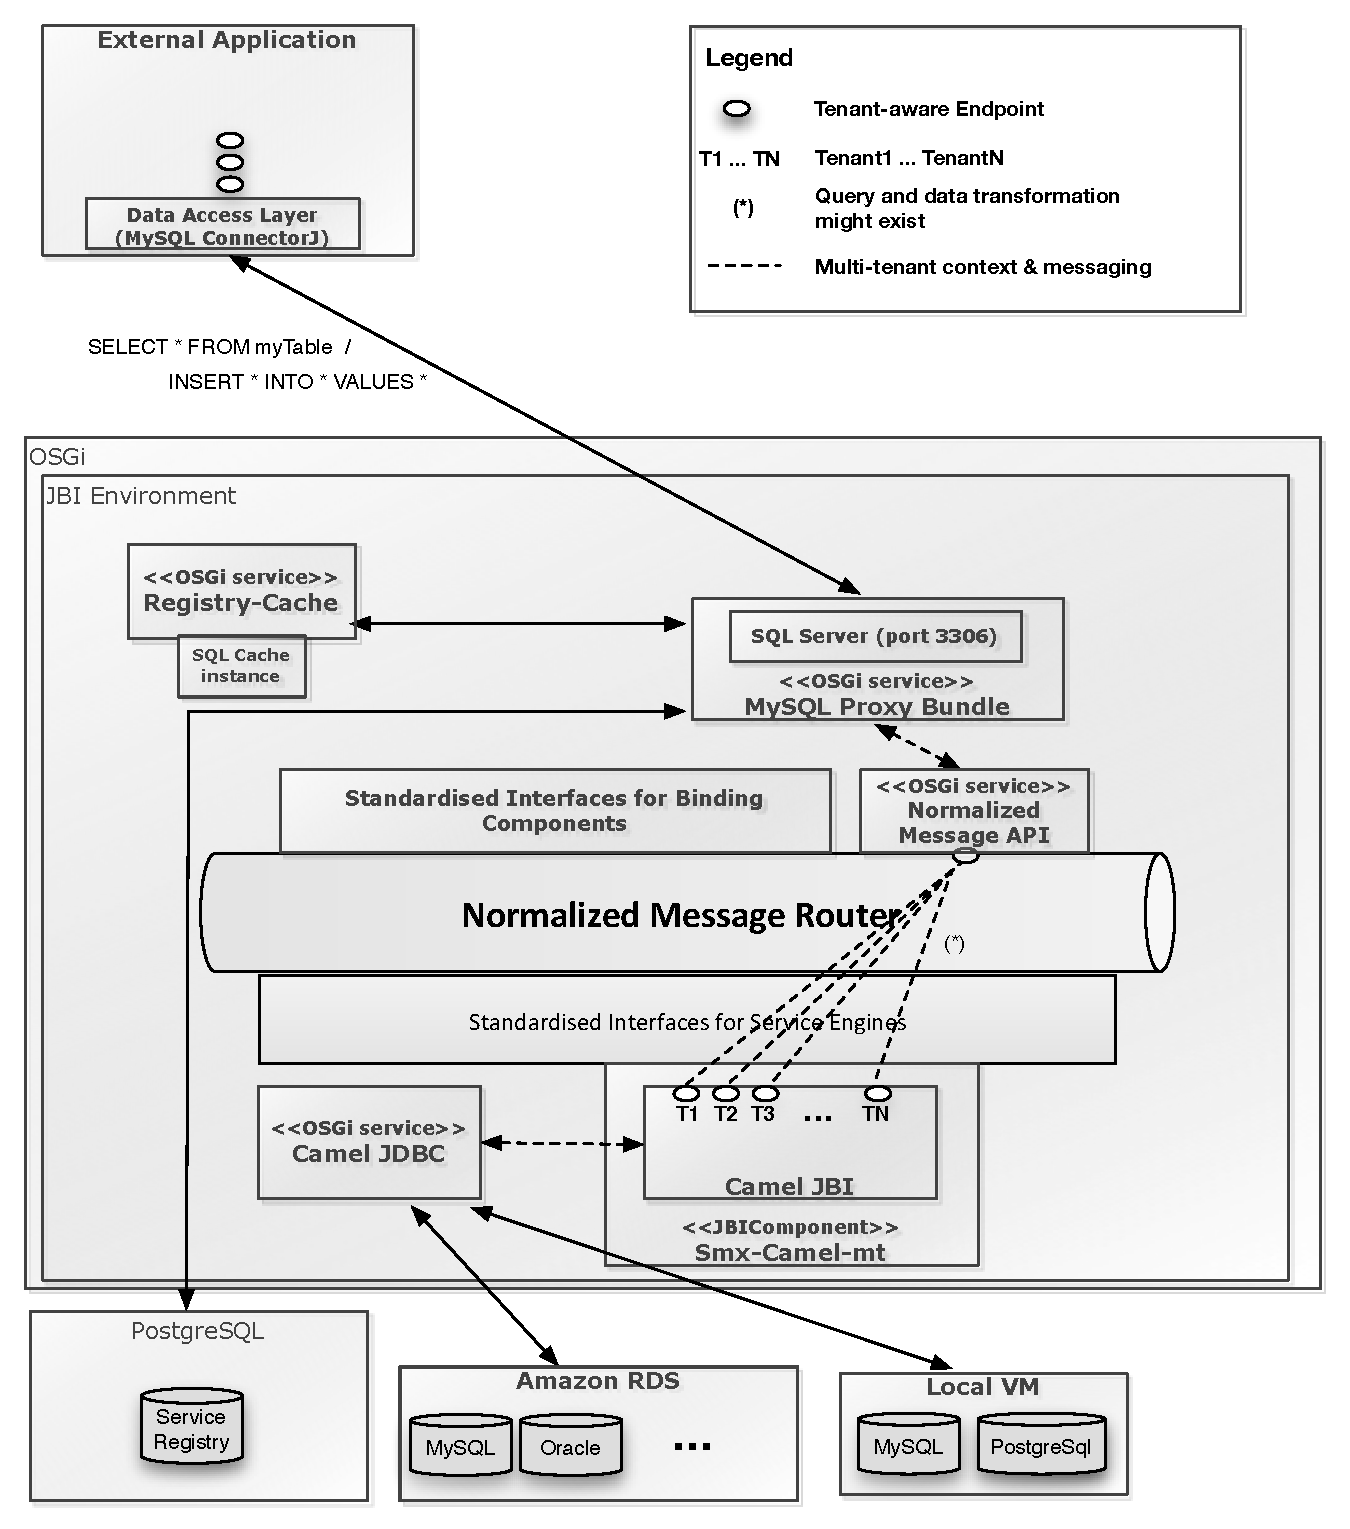
\includegraphics[clip, scale=0.6]{./gfx/sqlApproach/sqlApproachv2_doc.pdf}
	\caption[SQL Support Approach 1]{Architectural overview of the design approach one to support the MySQL communication protocol and routing to backend \ac{SQL} databases.}
	\label{fig:designsqlapp1}
\end{figure}

Apache Camel provides a set of components which integrate most of the communication technologies available in the market. Moreover, it provides an archetype for creating custom components we use in this diploma thesis. ServiceMix provides a Camel \ac{JBI} \ac{BC} which integrates the \ac{JBI} container with the camel router. Muhler extends this component in ServiceMix-mt and enriches it with multi-tenancy awareness. However, the supported multi-tenancy is at the level of tenants, and not at the level of tenant's users. We extend this component and provide user and tenant isolation between endpoints, by injecting the tenant and user UUID in the endpoint's URI (see Listing \ref{lst:endpointuri}). 

%%%%%%%%%%%%%%%%%%%%%%%%%%%%%
\lstinputlisting[float=htb,label={lst:endpointuri},caption={[Tenant-aware Endpoint Configuration]Extended Tenant-aware endpoint URI in extended Backus-Naur Form (EBNF) \cite{Muhler2012}.},style=ebnf]{./gfx/endpointconfiguration.txt}
%%%%%%%%%%%%%%%%%%%%%%%%%%%%%

With multi-tenancy at the tenant and user level, each user can deploy one \ac{JBI} tenant-aware endpoint in the ServiceMix-Camel-mt \ac{SE}. The routes deployed from each tenant-aware endpoint are performed under a different context, and an instance of the targeted component in the route is created. Therefore, with this approach we provide multi-tenancy at the messaging, endpoint, and routing and component context levels. 

Due to the lack of \ac{JDBC} support in ServiceMix for creating provider endpoints, we develop a custom camel component, and enrich it with \ac{JDBC} support for three database systems: MySQL, Oracle, and PostgreSQL. This component is extensible to more database systems when including its native driver, and is build as an \ac{OSGi} bundle and its packages are exported as an \ac{OSGi} service. Messages received from the \ac{NMR} are demarshaled to the backend database system communication protocol, and the response marshaled, correlated, and sent back to the MySQL Proxy Bundle. The demarshalers in this bundle provide the necessary support for transforming the \ac{NMF} response to a MySQL message.

As described in the previous section, ServiceMix-mt provides \ac{JBI} and \ac{OSGi} support and integration, but with some constraints. \ac{JBI} components cannot import packages from \ac{OSGi} bundles exporting its packages. The Servicemix-Camel-mt \ac{SE} provides integration with the camel router for a set of camel components. The camel manual specifies the need for adding statically the custom component packages in the \ac{JBI} \ac{SU} which contains the route definition. Therefore, this leads us to scalability problems in each of the \ac{SA} deployed by the tenants. The \ac{SA} size increases with the new supported database systems, and forces to redeploy all the \ac{SU}s containing the custom camel component when it is modified. This leads to management, storage capacity, and network capacity inconveniences. Hence, we provide a second, and final approach which is very similar to this one, but utilizing the ServiceMix-camel component deployed as \ac{OSGi} bundle. 

\FloatBarrier

\subsection{Approach 2}

In this second architectural design approach we address the scalability problems caused by the \ac{JBI} package dependencies in the \ac{SU}s described in the previous section. This approach is similar to the first one presented, and its main difference relies on the routing from the tenant-aware \ac{JBI} endpoints to the custom camel component \term{cdasmixjdbc} (see Figures \ref{fig:designsqlapp2} and \ref{fig:designsqlapp1}). The functionalities and operations in the MySQL proxy bundle do not differ with the previous approach.
 
\begin{figure}[htb]
	\centering
		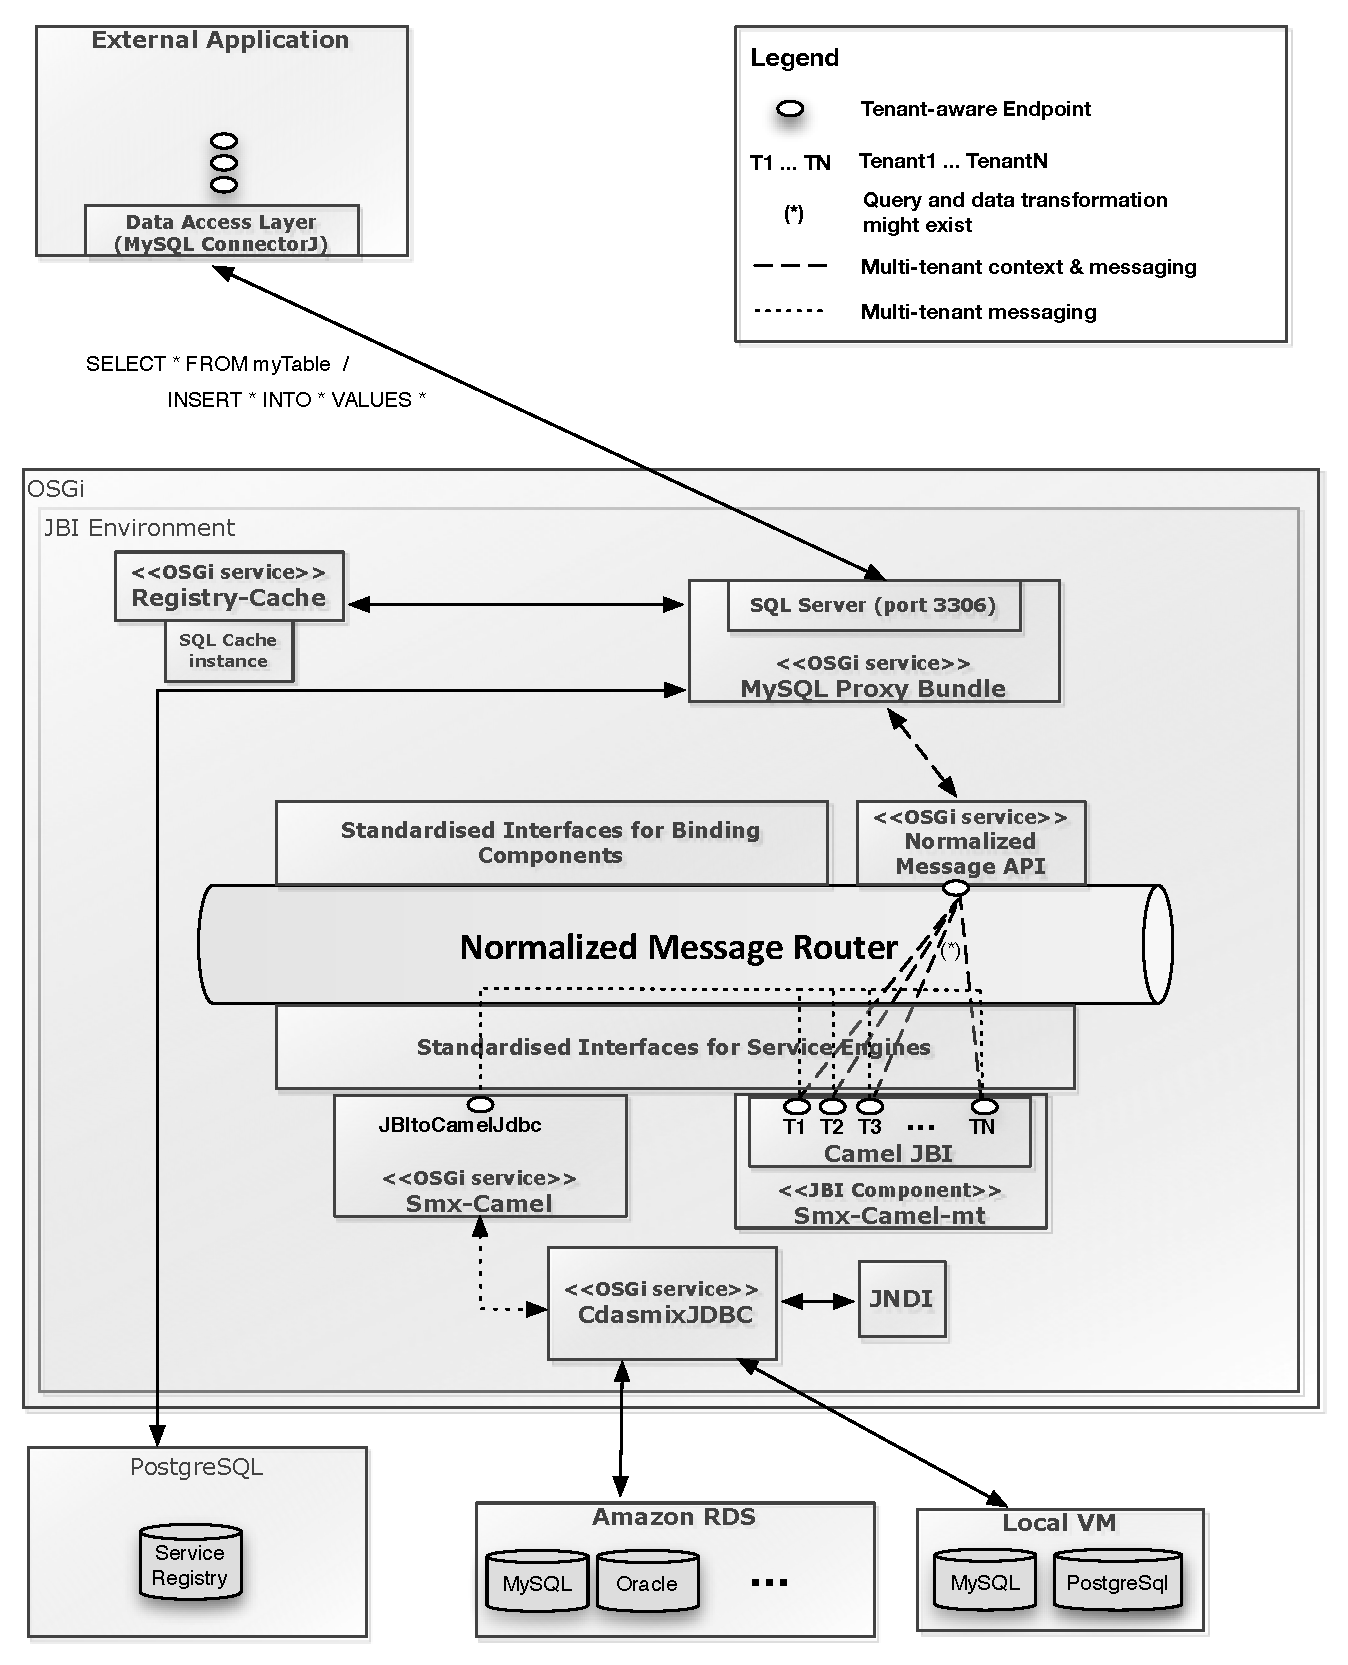
\includegraphics[clip, scale=0.6]{./gfx/sqlApproach/sqlApproachv3_doc.pdf}
	\caption[SQL Support Approach 2]{Architectural overview of the design approach two to support the MySQL communication protocol and routing to backend \ac{SQL} databases.}
	\label{fig:designsqlapp2}
\end{figure}

The message is routed from the MySQL proxy bundle to the tenant-aware \ac{JBI} endpoint deployed in ServiceMix-camel-mt. The multi-tenant message processor instance in ServiceMix-camel-mt routes the message to the \term{JBItoCamelJdbc} endpoint. 

As discussed before, the \ac{JBI} \ac{BC}s deployed in ServiceMix are \ac{OSGi} friendly. This means that the \ac{OSGi} contains a valid manifest file where the description of the bundle, import packages, and export packages are specified. \ac{SU}s deployed on this component are able to reference other \ac{OSGi} packages exposed as a service in the \ac{OSGi} service registry. We provide a single endpoint deployed in the ServiceMix-Camel component where the requests are sent to: the \term{JBItoCamelJdbc} endpoint. When the \term{JBItoCamelJdbc} endpoint is deployed on the ServiceMix-Camel \ac{OSGi} bundle, this searchs in the \ac{OSGi} container for the \term{CdasmixJDBC} component, and creates an instance of the component. Messages routed to the \term{JBItoCamelJdbc} endpoint are then forwarded to the \term{CdasmixJDBC} component, which selects the appropriate \ac{JDBC} native driver, creates a connection, demarshals the request, and forwards the request to the backend Cloud data store server. The connection is established after creating an instance of a \term{DataSource}, which is saved in the \ac{JNDI} registry for future connections, in order to avoid the creation of more than one \term{DataSource} instance per user per backend Cloud data store.

Responses retrieved from the backend Cloud data store are correlated with the initial request and routed back to the MySQL proxy bundle, which demarshals the retrieved data and sends it as a binary \ac{TCP} stream.

In this approach a new instance of the \term{cdasmixjdbc} is not created per tenant endpoint, but is shared between the tenants. Therefore, we cannot ensure an independent component context at the provider endpoint. However, messages contain the tenant information, and the \term{cdasmixjdbc} component interacts with the backend database system establishing separate \ac{JDBC} connections per request. Full multi-tenancy, at the levels of component creation, and endpoint level is not ensured, but it is ensured at the messaging, and context levels. Although full multi-tenancy is not supported, we avoid the deployment of \ac{SU}s which contain the \term{CdasmixJDBC} component in it, and whose size increase may lead to scalability problems in the system. Furthermore, we prevent the deployment of the same component n times, for the n multi-tenant aware endpoints, and prevent future management problems when modifying or upgrading the \term{CdasmixJDBC} component. 

\FloatBarrier



\section{NoSQL Databases}
\label{sec:fundamentalsnosqldb}  

\ac{RDBMS}s ensure data persistency over time and provide a wide set of features. However, the functionalities supported require a complexity, which is sometimes not needed for some applications, and harms important requirements in Web applications or in \ac{SOA} based applications, e.g. throughput. \ac{NoSQL} data stores aim to improve the efficiency of large amount of data storage while reducing its management cost \cite{nosqlcomputerworld}. NoSQL databases are designed to support horizontal scalability without relying on the highly available hardware \cite{strauchnosql}. In a Cloud storage environment where the user sees the available computing and storage resources as unlimited, a \ac{NoSQL} support in a Cloud storage environment might be adequate.

\ac{NoSQL} \ac{DBS} operate as a schema-less storage system, allowing the user to access, modify or freely insert his data without having to make first changes in the data structure \cite{nosql2012}. Cloud providers provide the users with an \ac{API} for accessing, modifying, and inserting data into his isolated container. For example, a user's Amazon Dynamo DB table and item can be accessed by its RESTful \ac{API}, or by installing at the user's side application the Amazon Web Services SDK \cite{amazondynamodb}. Furthermore, it provides the users through its Web-based management console the available management operations. 

Due to the growth of the \ac{NoSQL} support along different Cloud vendors, in this diploma thesis we provide a multi-tenant and transparent communication support for \ac{NoSQL} backend data stores in different Cloud providers. In the following sections we introduce the categorization of the different \ac{NoSQL} databases we aim to support in this diploma thesis, mentioning and giving examples of Cloud data stores available nowadays in the market.

\subsection{Key-value Databases}

In a key-value datastore elements are uniquely identified by an id, which the data store does not take into account its type, and are simply stored as a \ac{BLOB} . A user can get the value for the key, put a value for the key, or delete a key from the data store \cite{nosql2012}. Its storage model can be compared to a map/dictionary \cite{strauchnosql}. Products offering this data storage model in a Cloud infrastructure are Amazon DynamoDB \cite{amazondynamodb}, Google Cloud Storage \cite{googlecloudstorage}, Amazon SimpleDB  \cite{amazonsimpledb} , Amazon S3 \cite{amazons3}, etc. In this diploma thesis we mainly focus on the following key-value data stores: DynamoDB, and Google Cloud Storage.

Amazon DynamoDB's data model includes the following concepts: tables, items, and attributes \cite{amazondynamodb}. The attributes are a key-value, where the value is binary data. Attributes are stored in items, and these are stored in tables. Items stored in a table can be retrieved by referencing its unique id. The number of attributes is not limited by Amazon, but each item must have a maximum size of 64 KB. Accessing stored data in this data store can be mainly done in two ways: using the functionalities provided by the AWS SDK, or using the Cloud storage RESTful \ac{API}. 

Google Cloud Storage's data model includes the following concepts: buckets and objects \cite{googlecloudstorage}. Buckets contain on or more objects. The objects are identified within a bucket with its unique id. Users can perform I/O operations on both buckets and objects. For this purpose, Google Cloud storage provides RESTful \ac{API}.

In this diploma thesis we use an \ac{ESB} for accessing transparently tenant's databases migrated to the Cloud. Servicemix-mt provides multi-tenant \ac{HTTP} support \cite{gomez2012}. Therefore, we reuse and extend the multi-tenant \ac{HTTP} \ac{BC} in order to provide dynamic routing between the different data stores.

\subsection{Document Databases}

Document databases can be considered as a next step in improving the key-value storage model. In this storage model, documents are stored in the value part of the key-value store, making the value content examinable \cite{nosql2012}. Documents with different schemas are supported in the same collection, and can be referenced by the collection's key or by the document's attributes. One of the main difference in the attributes specification regarding \ac{RDBMS} is that in document stores document's attributes cannot be null. When there is an attribute without value, the attribute does not exist in the document's schema. Products implementing this data storage model are Apache CouchDB, MongoDB, etc. \cite{couchdb} \cite{mongodb}.

Mongo DB defines two storage structures: collections and documents \cite{mongodb}. A specific database contains one or more collections identified by its unique id. A specific collection stores one or more documents. Collections and documents stored in a database can be accessed, inserted and modified using the RESTful \ac{API} supported by the database system.

Apache CouchDB defines two storage structures: databases and documents. Data stored in CouchDB are \ac{JSON} documents. The main difference between this two described databases is that MongoDB implements a two step access to the documents: database, collection, and document. Apache CouchDB provides a RESTful \ac{API} for I/O operations.

This databases are not offered by Cloud providers like Amazon or Google, but as a software which can be deployed in user instances, e.g. Amazon EC2 AMI \cite{amazonec2}. 

\subsection{Column-family Stores}

One of the most known Column-family data stores is Cassandra. Column-family data stores store data in column families (groups of related columns which are often accessed together) as rows that have many columns associated with a row key \cite{nosql2012}. This approach allows to store and process data by column instead of by row, providing a higher performance when accessing large amount of data, e.g. allowing the application to access common accessed information in less time.

Cassandra has as its smallest unit of storage the column, which consists of a timestamp and a name-value pair where the name acts as a key \cite{nosql2012}. As in the relational model, a set of columns form up a row, which is identified by a key. A column family is a collection of similar rows. The main difference with the relational model is that each of the rows must not have the same columns, allowing the designer and the application consuming large amounts of data to customize the columns in each row, and the rows in each column family.

Cassandra is not shipped with a RESTful API for I/O operations. However, there are several open-source services layers for Cassandra, e.g. Virgil \cite{virgil}.

\FloatBarrier

\clearpage  